\subsection{Results Mapping}

\frame{
  \frametitle{Datasets and parameters}
  
\begin{tabular}{l|c|c|c|}
    Dataset & Plane test & Middlebury \cite{Middlebury}& Inhouse \\
    \hline
    \hline
    Ground truth & analytical & structured light & pattern matching \\ 
    Images & rectified & rectified & non rectified \\
    Calibration & +++ & ++ & + \\ 
    \hline
    \hline
    Mapping & yes & yes & yes \\ 
    Localization & yes & no & no \\
    \hline
    \hline
    Spline resolution & 20 x 20 & \multicolumn{2}{c|}{75 x 100} \\
    \hline
    Map dimensions & 0.9 x 1.2 & \multicolumn{2}{c|}{1.5 x 2.0} \\ 
    \hline
    Map resolution & \multicolumn{3}{c|}{90 x 120} \\ 
    \hline
  \end{tabular}
}

\subsection{Mapping}
\frame{\frametitle{Plane test case}
\begin{columns}
  \column{.5\textwidth}

  \begin{figure}[h!]
\centering
\resizebox{\linewidth}{!}{
  % This file was created by matlab2tikz.
%
%The latest updates can be retrieved from
%  http://www.mathworks.com/matlabcentral/fileexchange/22022-matlab2tikz-matlab2tikz
%where you can also make suggestions and rate matlab2tikz.
%
\definecolor{mycolor1}{rgb}{0.00000,0.44700,0.74100}%
\definecolor{mycolor2}{rgb}{0.85000,0.32500,0.09800}%
\definecolor{mycolor3}{rgb}{0.92900,0.69400,0.12500}%
\definecolor{mycolor4}{rgb}{0.49400,0.18400,0.55600}%
\definecolor{mycolor5}{rgb}{0.46600,0.67400,0.18800}%
%
\begin{tikzpicture}

\begin{axis}[%
width=0.969\linewidth,
height=0.75\linewidth,
at={(0\linewidth,0\linewidth)},
scale only axis,
xmin=-9,
xmax=5,
xlabel={Initialization [m]},
ymin=0,
ymax=35,
ylabel={No. Iterations},
axis background/.style={fill=white},
title style={font=\bfseries},
title={Convergence Study Plane Test},
legend style={at={(0.03,0.03)},anchor=south west,legend cell align=left,align=left,draw=white!15!black}
]
\addplot [color=mycolor1,line width=1.5pt,mark size=5.0pt,only marks,mark=o,mark options={solid}]
  table[row sep=crcr]{%
-0.2	6\\
0.2	4\\
-0.4	7\\
0.4	3\\
-0.6	17\\
0.6	2\\
-0.8	30\\
0.8	2\\
-1	30\\
1.2	1\\
2.2	30\\
1.4	1\\
2.4	30\\
1.6	1\\
2.6	30\\
1.8	6\\
2.8	30\\
};
\addlegendentry{b=1};

\addplot [color=mycolor2,line width=1.5pt,mark size=5.0pt,only marks,mark=x,mark options={solid}]
  table[row sep=crcr]{%
-20	30\\
-15	30\\
-10	30\\
-5	30\\
0	4\\
1	2\\
2	20\\
-4	25\\
-3	26\\
-2	24\\
-1	7\\
1.2	1\\
2.2	30\\
1.4	1\\
2.4	30\\
1.6	1\\
2.6	30\\
1.8	4\\
2.8	30\\
-7	30\\
-5	30\\
-4	25\\
-3	26\\
-0.2	4\\
0.2	3\\
-0.4	6\\
0.4	2\\
-0.6	6\\
0.6	2\\
-0.8	6\\
0.8	2\\
};
\addlegendentry{b = 100};

\addplot [color=mycolor3,line width=1.5pt,mark size=5.0pt,only marks,mark=asterisk,mark options={solid}]
  table[row sep=crcr]{%
-20	30\\
-10	30\\
-5	30\\
-3	30\\
0	4\\
1	1\\
2	30\\
-1	7\\
1.2	1\\
2.2	30\\
1.4	1\\
2.4	30\\
1.6	1\\
2.6	30\\
1.8	4\\
2.8	30\\
-0.2	4\\
0.2	3\\
-0.4	6\\
0.4	2\\
-0.6	6\\
0.6	2\\
-0.8	7\\
0.8	2\\
};
\addlegendentry{b = 1000};

\addplot [color=mycolor4,solid,line width=1.5pt]
  table[row sep=crcr]{%
3	0\\
3	35\\
};
\addlegendentry{Camera location};

\addplot [color=mycolor5,solid,line width=1.5pt]
  table[row sep=crcr]{%
1.3178	0\\
1.3178	35\\
};
\addlegendentry{Plane location};

\end{axis}
\end{tikzpicture}%
}
\end{figure}
  \column{.5\textwidth}

    \begin{figure}[H]
    \begin{subfigure}{.2\linewidth}
      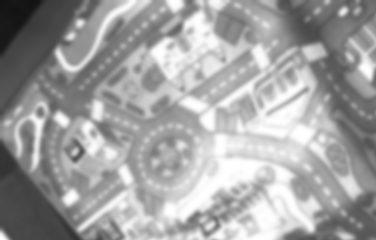
\includegraphics[width=\textwidth]{figures/planetest1.png}
    \end{subfigure}
    \begin{subfigure}{.2\linewidth}
      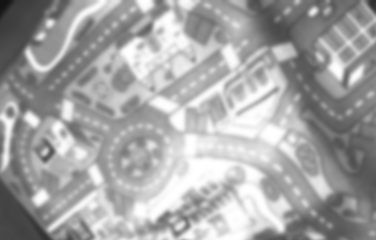
\includegraphics[width=\textwidth]{figures/planetest2.png}
    \end{subfigure}
  \end{figure}

  \begin{figure}[H]
    \centering
    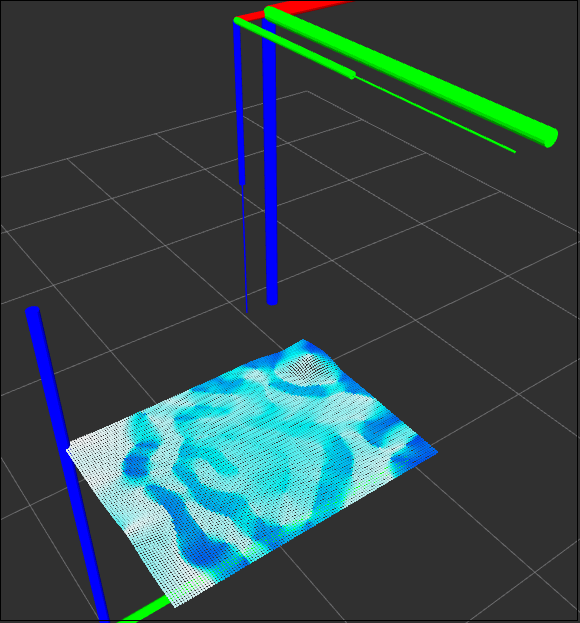
\includegraphics[width=.9\linewidth]{figures/planetest3d.png}
  \end{figure}
\end{columns}
}

%\frame{\frametitle{Simulation test case}}
\frame{
  \frametitle{Middlebury dataset}
  
  \begin{figure}[H]
  \begin{subfigure}{.2\linewidth}
    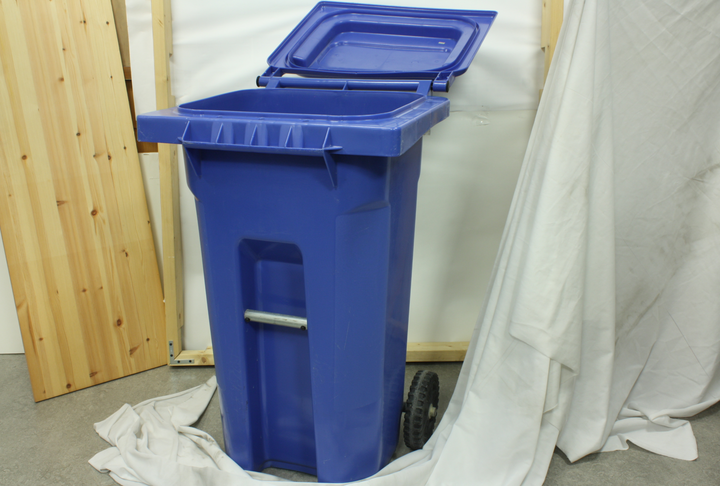
\includegraphics[width=\textwidth]{figures/recycle0.png}
  \end{subfigure}
  \begin{subfigure}{.2\linewidth}
    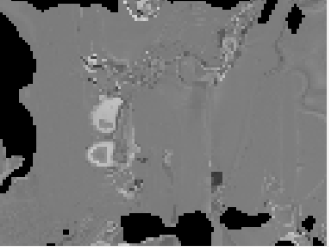
\includegraphics[width=\textwidth]{figures/middlebury_residuals_b1.png}
  \end{subfigure}
  \begin{subfigure}{.2\linewidth}
    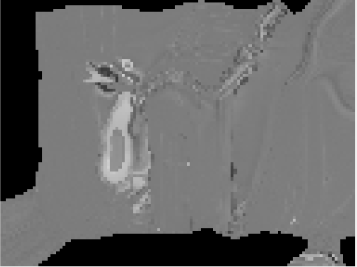
\includegraphics[width=\textwidth]{figures/middlebury_residuals_b10.png}
  \end{subfigure}
  \end{figure}
  
  \begin{figure}[H]
  \begin{subfigure}{.2\linewidth}
    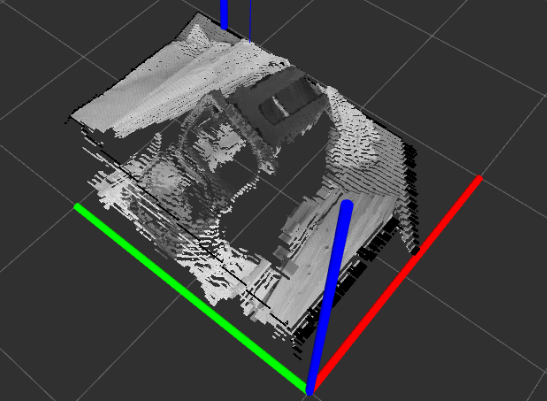
\includegraphics[width=\textwidth]{figures/middlebury_3d_groundtruth.png}
  \end{subfigure}
  \begin{subfigure}{.2\linewidth}
    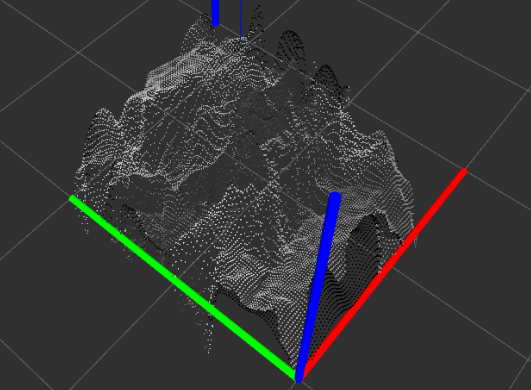
\includegraphics[width=\textwidth]{figures/middlebury_3d_b1.png}
  \end{subfigure}
  \begin{subfigure}{.2\linewidth}
    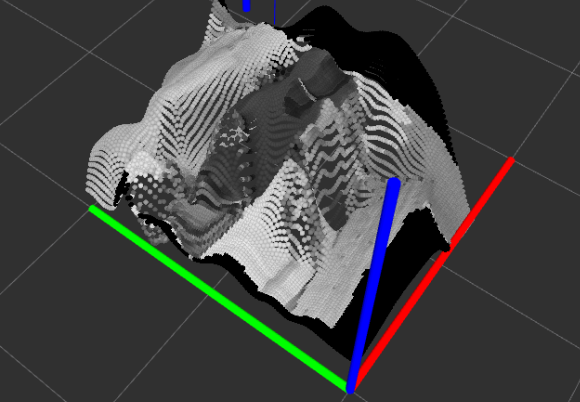
\includegraphics[width=\textwidth]{figures/middlebury_3d_b10.png}
  \end{subfigure}
  \end{figure}
  
  \begin{figure}[H]
  \begin{subfigure}{.2\linewidth}
    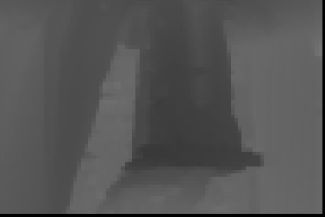
\includegraphics[width=\textwidth]{figures/middlebury_disparity.png}
  \end{subfigure}
  \begin{subfigure}{.2\linewidth}
    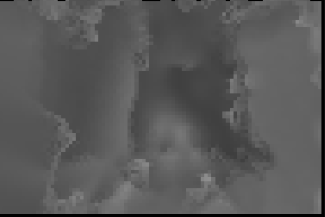
\includegraphics[width=\textwidth]{figures/middlebury_disparity_b1.png}
  \end{subfigure}
  \begin{subfigure}{.2\linewidth}
    
\includegraphics[width=\textwidth]{figures/middlebury_disparity_b10.png}
  \end{subfigure}
  \end{figure}

}

\frame{
  \frametitle{Inhouse dataset}

  Parameters: 
  $\beta = 10$
  $\gamma = 100e3$
  $d = 100$

  \scalebox{.9}{
    \begin{tabularx}{\textwidth}{X c c c}
  Parameters: \newline
  $\beta = 10$ \newline
  $\gamma = 1e6$ \newline
  $d = 100$ &
    \multirow{2}{*}{
    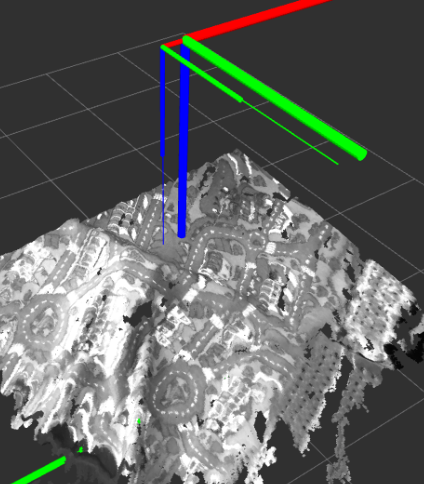
\includegraphics[valign=t,width=.25\textwidth]{figures/bag_far_gt.png}
    } &
    \multirow{2}{*}{
    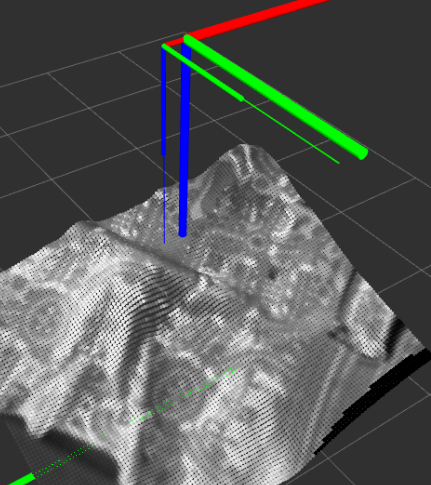
\includegraphics[valign=t,width=.25\textwidth]{figures/bag_far_map.png}
    } &
    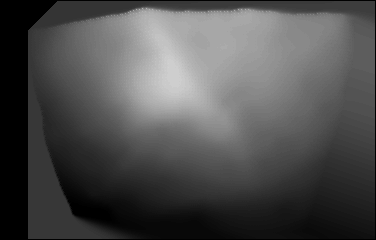
\includegraphics[valign=t,width=.2\textwidth]{figures/disparity_map_far_hr.png} \\
    & & &
    
\includegraphics[valign=t,width=.2\textwidth]{figures/disparity_gt_far.png} \\
    & \multirow{2}{*}{
    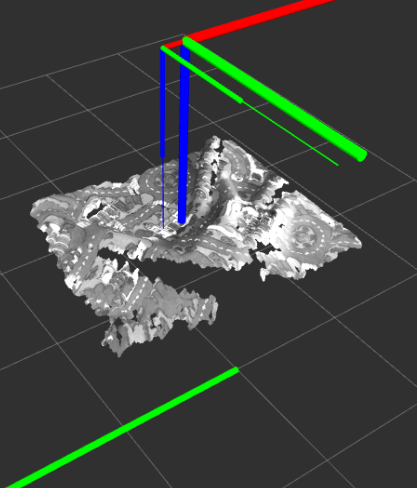
\includegraphics[valign=t,width=.25\textwidth]{figures/bag_close_gt.png} 
    } &
    \multirow{2}{*}{
    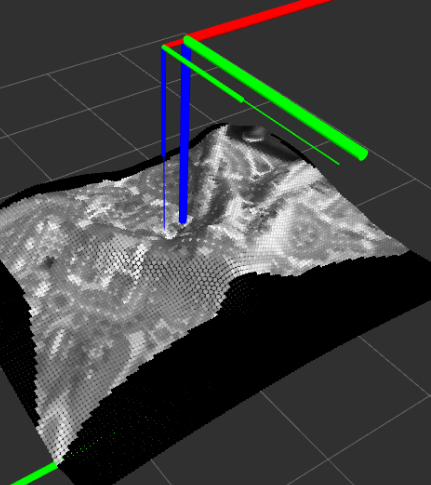
\includegraphics[valign=t,width=.25\textwidth]{figures/bag_close_map.png} 
    } &
    
\includegraphics[valign=t,width=.2\textwidth]{figures/disparity_map_close_hr.png} \\
    & & &
    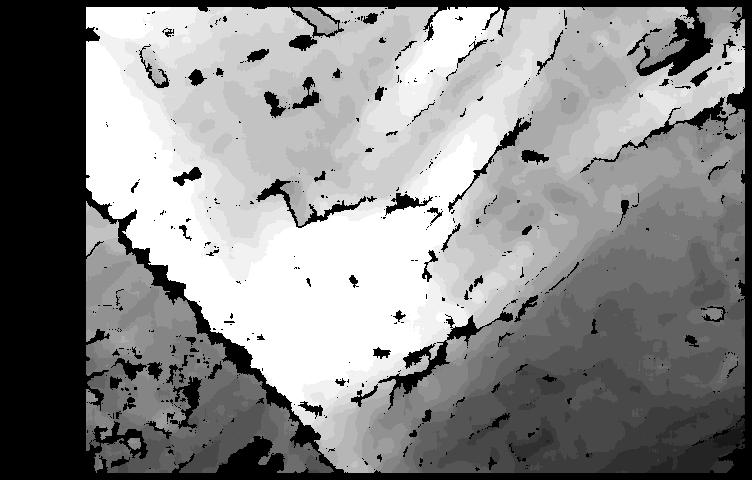
\includegraphics[valign=t,width=.2\textwidth]{figures/disparity_gt_close.png} \\
  \end{tabularx}
}

}

\subsection{Localization}
\frame{\frametitle{Plane test case}}

%\frame{\frametitle{Simulation test case}}
